\chapter{Simulator Models}

\section{Basic Components}

Every component is a part of the class "BaseComponent", which has as variables the name of the component and the nodes on which they are connected. Furthermore, four functions are defined in "BaseComponent":

\begin{itemize}
\item "init": This function initializes the values of the component variables. For  instance, initial values of current and voltage of inductors and capacitors.

\item "applySystemMatrixStamp": This function stamps the conductance matrix $G$.

\item "applyRightSideMatrixStamp": This function stamps the vector $A$.

\item "step": This function updates the values of the vector $A$ in each calculation step.

\item "postStep": This function updates the variables which depends on the solution of the equation $e=G^{-1} \cdot A$.
\end{itemize}

\subsection{Linear Resistor}
The linear resistor has the following parameters defined by the user:
\begin{itemize}
\item name: Name of the component
\item src: First node where the resistor is connected
\item dest: Second node where the resistor is connected
\item resistance: Resistance given in Ohms
\end{itemize}

The function "applySystemMatrixStamp" stamps the resistance to the conductance matrix $G$ as in section \ref{ResistorMatrixStamp} considering $j=src$ and $k=dest$.


\subsection{Inductor}

The inductor model is developed based on the Resistive Companion Method presented in section \ref{ResistiveCompanion}.

For a constant frequency and fixed time step, the value of $R_L$ will be constant. Therefore, the matrix stamp of the conductance matrix will be made just once. By the other hand, the value of $A_L$ needs to be updated each step, since it depends on the voltage and current of the inductor at the previous step.

The inductor has the following parameters defined by the user:

\begin{itemize}
\item name: Name of the component
\item src: First node where the inductor is connected
\item dest: Second node where the inductor is connected
\item inductance: Inductance given in H
\end{itemize}

The function "applySystemMatrixStamp" will stamp $R_L$ to the conductance matrix $G$ as in subsection, considering $j=src$ and $k=dest$. \ref{ResistiveCompanionInductor}

The function "init" defines as zero the initial values of current and voltage of the inductor as well the initial value of the equivalent current source $A_L$.

\begin{align*}
v_L(0)&=0V \\
i_L(0)&=0A \\
A_L(0)&=0A \\
\end{align*}

The function "step" is called each step. It recalculates the value of the equivalent current source $A_L(k)$, using equation \ref{eq:AL} and apply the stamp of the vector $A$ as in subsection \ref{ResistiveCompanionInductor}, considering $j=src$ and $k=dest$.

The function "poststep" will calculate the inductor voltage $v_L$, based on the solution of the vector $e$ at the actual step (k+1) and the inductor current, based on the calculated $v_L$ and on the value of $A_L$ from the previous step (k).

\begin{equation} \label{eq:inductorVoltage}
v_L(k+1) = e_{src}(k+1) - e_{dest}(k+1)
\end{equation}

\begin{equation} \label{eq:inductorCurrent}
i_L(k+1) = \frac{v_L(k+1)}{R_L} + A_L(k)
\end{equation}
 

\subsection{Capacitor}

The capacitor model is also developed based on the Resistive Companion Method and is similar to the inductor model.

It has the following parameters defined by the user:

\begin{itemize}
\item name: Name of the component
\item src: First node where the inductor is connected
\item dest: Second node where the inductor is connected
\item capacitance: Capacitance given in F
\end{itemize}

The function "applySystemMatrixStamp" will stamp $R_C$ to the conductance matrix $G$ as in subsection \ref{ResistiveCompanionCapacitor}, considering $j=src$ and $k=dest$.

The function "init" defines as zero the initial values of current and voltage of the capacitor as well the initial value of the equivalent current source $A_C$.

\begin{align*}
v_C(0)&=0V \\
i_C(0)&=0A \\
A_C(0)&=0A \\
\end{align*}

The function "step" is called each time step. It recalculates the value of the equivalent current source $A_C(k)$ as in equation \ref{eq:AC} and stamps its value to the vector $A$ as in subsection \ref{ResistiveCompanionCapacitor}, considering $j=src$ and $k=dest$.

The function "poststep" will calculate the capacitor voltage $v_C$, based on the solution of $e$ at the actual step (k+1) and the capacitor current, based on the calculated $v_C(k+1)$ and on the value of $A_C$ from the previous step (k).

\begin{equation}
v_C(k+1) = e_{src}(k+1) - e_{dest}(k+1)
\end{equation}

\begin{equation}
i_C(k+1) = \frac{v_C(k+1)}{R_C} - A_C(k)
\end{equation}
 

\subsection{Real Voltage Source} \label{sub:RealVoltageSource}

A real voltage source can be represented as a voltage source $V$ in series with a resistance $R$, with

\begin{equation}
V=Va \cdot cos(\omega t + \phi)
\end{equation}
In dynamic phasors the voltage source V becomes

\begin{equation}
V = Va \cdot cos (\phi) + jVa \cdot sin(\phi) 
\end{equation}

As nodal analysis does not support voltage source, it is transformed to a current source using the Norton Equivalent as shown in figure \ref{fig:Real_Voltage_Source}.

\begin{figure}[ht]
	\centering
	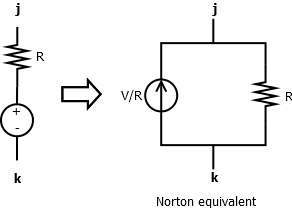
\includegraphics[scale=0.6]{img/RealVoltageSource.png} 
	\caption{Real Voltage Source}
	\label{fig:Real_Voltage_Source}
\end{figure}

The matrix stamp for a real voltage source is therefore as in equation \ref{eq:MatrixStampRealVS}.

\begin{align} \label{eq:MatrixStampRealVS}
\begin{split}
&
\begin{matrix}
& \cdots & j & \quad k & \cdots
\end{matrix}\\[-6pt]
\begin{matrix}
\vdots\\[6pt]
j\\[6pt]
k\\[6pt]
\vdots\\
\end{matrix}
&
\begin{bmatrix}
	\quad & \quad &  \\[6pt]
	\quad & \dfrac{1}{R} & \dfrac{-1}{R} & \quad  \\[6pt]
	\quad & \dfrac{-1}{R} & \dfrac{1}{R} & \quad \\[6pt]
	\quad &  & 
\end{bmatrix}
\begin{bmatrix}
	\quad \\[6pt]
	e_j(k+1)\\[6pt]
	e_k(k+1)\\[6pt]
	\quad
\end{bmatrix}
=
\begin{matrix}
\vdots\\[6pt]
j\\[6pt]
k\\[6pt]
\vdots\\
\end{matrix}
\begin{bmatrix}
	\quad \\[6pt]
	\dfrac{V}{R} \\[6pt]
	-\dfrac{V}{R} \\[6pt]
	\quad
\end{bmatrix}
\end{split}
\end{align}

The following parameters are defined by the user for the real voltage source:

\begin{itemize}
\item name: Name of the component
\item src: Node connected to voltage source positive terminal (j)
\item dest: Node connected to voltage source negative terminal (k)
\item voltage: Voltage in V
\item phase: Phase shift in degrees
\item resistance: Series resistance in ohms 
\end{itemize}

The function "applySystemMatrixStamp" will stamp the resistance at the conductance matrix $G$.
The function "applyRightSideVectorStamp" will stamp the equivalent current source $I=\frac{V}{R}$ to the vector $A$.
The function "step" will repeat the stamp of the vector $A$ each time step.

\subsection{Ideal Voltage Source}

The model of the ideal voltage source uses the modified nodal analysis as presented in subsection \ref{IdealVoltageSource}.
The following parameters are defined by the user:

\begin{itemize}
\item name: Name of the component
\item src: Node connected to voltage source positive terminal
\item dest: Node connected to voltage source negative terminal
\item voltage: Voltage in V
\item phase: Phase shift in degrees
\item num: Number of the voltage source (the voltage sources have to be numbered in sequence) 
\end{itemize}

The function "applyMatrixStamp" will stamp the conductance matrix according to subsection \ref{IdealVoltageSource}. The additional unknown $i_{jk}$ of the voltage source number 1 (with variable num=1) will be added in the first line after the last node voltage and so on. Therefore, for a circuit with n voltage sources and m nodes, the vector of unknown variable $e$ and the vector $A$ will have the size $m+n$. The conductance matrix G will have the size $(m+n)X(m+n)$.

\begin{equation}
	e=
	\begin{bmatrix}
		e_1 \\
		\vdots \\
		e_m \\
		i_1 \\
		\vdots \\
		i_n
	\end{bmatrix}
\end{equation}

The function "applyRightSideVectorStamp" will stamp the voltage at the corresponding line of the vector $A$.
The function step will repeat the stamp of the vector $A$ each time step.

\subsection{Current Source}

For the current source, the following parameters are defined by the user:

\begin{itemize}
\item name: Name of the component
\item src: Node connected to current source positive terminal
\item dest: Node connected to current source negative terminal
\item current: Current in A
\item phase: Phase shift in degrees
\end{itemize}

The function "applyRightSideVectorStamp" will stamp the current at the vector $A$ as in subsection \ref{CurrentSourceMatrixStamp}.

\subsection{RX Line}
The RX Line model corresponds to a resistance in series with a inductance. The inductance is represented using resistive companion and therefore replaced by a resitance in parallel to a current source.

The user can define the RX Line in two ways. The first one is with the following parameters:

\begin{itemize}
\item name: Name of the component
\item node1: First node, where the resistance is connected
\item node2: Second node, where the inductance is connected
\item node3: Node between resistance and inductance 
\item resistance: Resistance in ohms
\item inductance: Inductance in H
\end{itemize}

\begin{figure}[h]
	\centering
	\includegraphics[scale=0.5]{img/RxLine.png} 
	\caption{RX Line model}
	\label{fig:RxLine}
\end{figure}

In this case, the function "applySystemMatrixStamp" will stamp the resistances $R$ between node1 and node3 and $R_L$ between node3 and node2 to the conductance matrix $G$. The function "step" will recalculate the value of $A_L$ as in equation \ref{eq:AL} and stamp it between node3 and node2 to the vector $A$. The function "poststep" will update the values of inductor current and voltage using equations \ref{eq:inductorCurrent} and \ref{eq:inductorVoltage}.

\begin{align}
\begin{split}
&
\begin{matrix}
& \cdots & node1 & node2 &  node3 & \cdots
\end{matrix}\\[-6pt]
G \quad = \quad
\begin{matrix}
\vdots\\[8pt]
node1\\[8pt]
node2\\[8pt]
node3\\[8pt]
\vdots\\
\end{matrix}
&
\begin{bmatrix}
	\quad & \quad &  \\[8pt]
	\quad & \quad \dfrac{1}{R} & \quad & \quad \dfrac{-1}{R} & \quad  \\[8pt]
	\quad & \quad & \quad \dfrac{1}{R_L} & \quad \dfrac{-1}{R_L} & \quad \\[8pt]
	\quad & \quad \dfrac{-1}{R} & \quad \dfrac{-1}{R_L} & \dfrac{1}{R}+\dfrac{1}{R_L} & \quad\\[8pt]
	\quad\\ 
\end{bmatrix}
\end{split}
\end{align}
\begin{align}
\begin{split}
A\quad = \quad
\begin{matrix}
\vdots\\[8pt]
node1\\[8pt]
node2\\[8pt]
node3\\[8pt]
\vdots\\
\end{matrix}
\begin{bmatrix}
	\quad \\[8pt]
	\quad \\[8pt]
	A_L(k) \\[8pt]
	-A_L(k) \\[8pt]
	\quad
\end{bmatrix}
\end{split}
\end{align}

The second way of define the RX Line is defining only two nodes (node1 and node2). In this case, the equivalent circuit in figure \ref{fig:RxLine2} is considered.

\begin{figure}[ht]
	\centering
	\includegraphics[scale=0.5]{img/RxLine2.png} 
	\caption{RX Line model with two nodes}
	\label{fig:RxLine2}
\end{figure}

The function "applySystemMatrixStamp" will stamp the resistance $R+R_L$ between node1 and node2 to the conductance matrix $G$.

\begin{align}
\begin{split}
&
\begin{matrix}
& \cdots & node1 & \quad node2 & \cdots
\end{matrix}\\[-5pt]
G \quad = \quad
\begin{matrix}
\vdots\\[6pt]
node1\\[6pt]
node2\\[6pt]
\vdots\\
\end{matrix}
&
\begin{bmatrix}
	\quad & \quad &  \\[6pt]
	\quad & \dfrac{1}{R+R_L} & \dfrac{-1}{R+R_L} & \quad  \\[6pt]
	\quad & \dfrac{-1}{R+R_L} & \dfrac{1}{R+R_L} & \quad \\[6pt]
	\quad &  & 
\end{bmatrix}
\end{split}
\end{align}

The function "step" will update the values of $A_L$ as in equation \ref{eq:AL} and $A_{Leq}(k)$. $A_{Leq}$ will be stamped to the vector $A$ as in equation \ref{eq:AleqStamp}.

\begin{equation}
A_{Leq}(k)=A_L(k) \cdot \frac{R_L}{R_L+R}
\end{equation}

\begin{align} \label{eq:AleqStamp}
\begin{split}
A\quad = \quad
\begin{matrix}
\vdots\\[8pt]
node1\\[8pt]
node2\\[8pt]
\vdots\\
\end{matrix}
\begin{bmatrix}
	\quad \\[8pt]
	-A_{Leq}(k) \\[8pt]
	A_{Leq}(k) \\[8pt]
	\quad
\end{bmatrix}
\end{split}
\end{align}

The function "poststep" will calculate the values of the line voltage and current and inductor voltage and current for the actual step (k+1).

\begin{equation}
	v_{Line}(k+1) = v_{node1}(k+1) - v_{node2}(k+1) 
\end{equation}

\begin{equation}
	i_{Line}(k+1) = \frac{v_{Line}(k+1)}{R+R_L} + A_{Leq} 
\end{equation}

\begin{equation}
	v_L(k+1) = v_{Line}(k+1) - R \cdot i_{Line}(k+1)
\end{equation}

\begin{equation}
	i_L(k+1) = i_{Line}(k+1)
\end{equation}

In both cases, the function "init" is setting every initial value to zero.

\subsection{Pi Line}
The Pi Line model corresponds to a resistance in series with a inductance and two shunt capacitors as shown in figure \ref{fig:PiLine}. The inductance and the capacitance are represented using resistive companion and therefore replaced by a resitance in parallel to a current source.

The following parameters are defined by the user:

\begin{itemize}
\item name: Name of the component
\item node1: First node, where the resistance and the first capacitor are connected
\item node2: Second node, where the inductance and the second capacitor are connected
\item node3: Node between resistance and inductance 
\item resistance: Resistance in ohms
\item inductance: Inductance in H
\item capacitance: Capacitance in F
\end{itemize}

\begin{figure}[h]
	\centering
	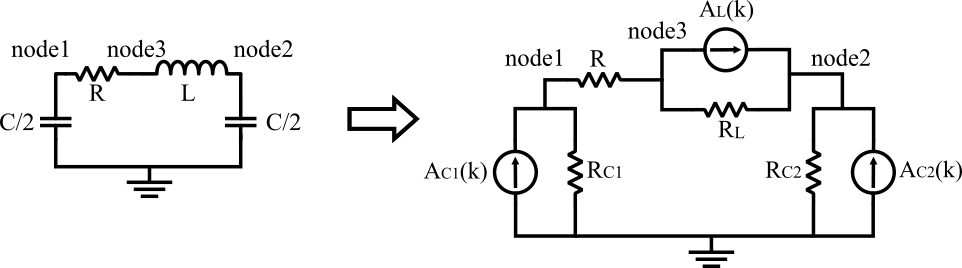
\includegraphics[scale=0.5]{img/PiLine.png} 
	\caption{Pi Line model}
	\label{fig:PiLine}
\end{figure}

The function "init" will initialize all currents and voltages with zero.

The function "applySystemMatrixStamp" will stamp the resistances $R$ between node1 and node3, $R_L$ between node3 and node2, $R_{C1}$ between node1 and reference node and $R_{C2}$ between node2 and reference node to the conductance matrix $G$.

The function "step" will recalculate the value of $A_L$, $A_{C1}$ and $A_{C2}$ and stamp it to the vector $A$.

The function "poststep" will update the values of inductor and capacitors current and voltage.

\begin{align}
\begin{split}
&
\begin{matrix}
& \quad \cdots & \quad node1 \quad & \quad node2 \quad &  \quad node3 & \cdots
\end{matrix}\\[-6pt]
G \quad = \quad
\begin{matrix}
\vdots\\[8pt]
node1\\[8pt]
node2\\[8pt]
node3\\[8pt]
\vdots\\
\end{matrix}
&
\begin{bmatrix}
	\quad & \quad &  \\[8pt]
	\quad & \quad \dfrac{1}{R} + \dfrac{1}{R_{C1}} & \quad & \quad \dfrac{-1}{R} & \quad  \\[8pt]
	\quad & \quad & \quad \dfrac{1}{R_L} + \dfrac{1}{R_{C2}} & \quad \dfrac{-1}{R_L} & \quad \\[8pt]
	\quad & \quad \dfrac{-1}{R} & \quad \dfrac{-1}{R_L} & \dfrac{1}{R}+\dfrac{1}{R_L} & \quad\\[8pt]
	\quad\\ 
\end{bmatrix}
\end{split}
\end{align}
\begin{align}
\begin{split}
A\quad = \quad
\begin{matrix}
\vdots\\[8pt]
node1\\[8pt]
node2\\[8pt]
node3\\[8pt]
\vdots\\
\end{matrix}
\begin{bmatrix}
	\quad \\[8pt]
	A_{C1}(k) \\[8pt]
	A_L(k) + A_{C2}(k) \\[8pt]
	-A_L(k) \\[8pt]
	\quad
\end{bmatrix}
\end{split}
\end{align}
 
\section{Synchronous Machine}

The model is according to \cite{wang2010methods} and \cite{kundur1994power}. 

\subsubsection{Prerequisites}


\subsubsection{Magnetic Circuits}

Considering the magnetic circuit of figure \ref{fig:MagneticCircuit} with two magnetically coupled windings with number of turns $N_1$ and $N_2$, resistance $r_1$ and $r_2$ and currents $i_1$ and $i_2$ respectively, the flux linkage with the respective windings, produced by the total effect of both currents are given by equations \ref{eq:FluxLinkage1} and \ref{eq:FluxLinkage2}.

\begin{equation} \label{eq:FluxLinkage1}
	\lambda_1 = N_1(\Phi_{l1} + \Phi_{m1} + \Phi_{m2})
\end{equation}
\begin{equation} \label{eq:FluxLinkage2}
	\lambda_2 = N_2(\Phi_{l2} + \Phi_{m2} + \Phi_{m1})
\end{equation}
\\
where

$\Phi_{m1}$ is the mutual flux linking both windings due to current $i_1$;

$\Phi_{m2}$ is the mutual flux linking both windings due to current $i_2$;

$\Phi_{l1}$ is the leakage flux linking winding 1 only;

$\Phi_{l2}$ is the leakage flux linking winding 2 only.

\begin{figure}[h]
	\centering
	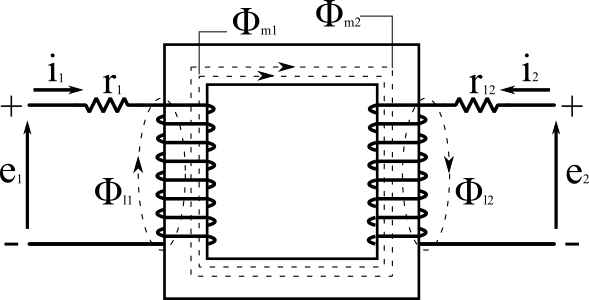
\includegraphics[scale=0.6]{img/MagneticCircuit.png} 
	\caption{Magnetically coupled circuit}
	\label{fig:MagneticCircuit}
\end{figure}

The flux linkage can also be expressed in terms of self and mutual inductance as in equation \ref{eq:FluxLinkageInductances}

\begin{equation} \label{eq:FluxLinkageInductances}
	\begin{bmatrix}
		\lambda_1\\
		\lambda_2
	\end{bmatrix}
		=
	\begin{bmatrix}
		L_{11} & L_{12}\\
		L_{21} & L_{22}
	\end{bmatrix}
		\cdot
	\begin{bmatrix}
		i_1\\
		i_2		
	\end{bmatrix}
\end{equation}
\\
where $L_{11}$ and $L_{22}$ are the self inductances of windings 1 and 2 respectively and defined as the flux linkage per unit current in the same winding. $L_{12}$ and $L_{21}$ are the mutual inductance between two windings, defined as the flux linkage with one winding per unit current in the other winding.

\begin{equation}
	L_{11} = \frac{N_1(\Phi_{m1} + \Phi_{l1})}{i_1}
\end{equation}
\begin{equation}
	L_{22} =  \frac{N_2(\Phi_{m2} + \Phi_{l2})}{i_2}
\end{equation}

\begin{equation}
	L_{12} = \frac{N_1 \Phi_{m2}}{i_2}
\end{equation}
\begin{equation}
	L_{21} = \frac{N_2 \Phi_{m1}}{i_1}
\end{equation}

The mutual fluxes $\Phi_{m1}$ and $\Phi_{m2}$ can be defined as in equations \ref{eq:MutualFlux1} and \ref{eq:MutualFlux2}, where $\Re_m$ is the reluctance of the path of the magnetizing fluxes. 

\begin{equation} \label{eq:MutualFlux1}
	\Phi_{m1} = \frac{N_1 i_1}{\Re_m} 
\end{equation} 
\begin{equation} \label{eq:MutualFlux2}
	\Phi_{m2} = \frac{N_2 i_2}{\Re_m} 
\end{equation}

From these equations, it is possible to see that

\begin{equation}
	L_{12}=L_{21}= \frac{N_1 N_2}{\Re_m}
\end{equation}

The terminal voltages $e_1$ and $e_2$ are defined as following:

\begin{equation} \label{eq:VoltageEquation1}
	e_1 = \frac{d \lambda_1}{d t} + r_1 i_1
\end{equation}
\begin{equation} \label{eq:VoltageEquation2}
	e_2 = \frac{d \lambda_2}{d t} + r_2 i_2
\end{equation}

Equations \ref{eq:FluxLinkageInductances}, \ref{eq:VoltageEquation1} and \ref{eq:VoltageEquation2} give the performance of the magnetically coupled circuit.

\subsubsection{Park's transformation}

Park's transformation is commonly used to achieve a model with static parameters:
%
\begin{equation}
\mathbf{K_s} = \frac{2}{3}
 \begin{bmatrix} 
  \cos \theta & \cos(\theta-\frac{2\pi}{3}) & \cos(\theta+\frac{2\pi}{3}) \\
  \sin \theta & \sin(\theta-\frac{2\pi}{3}) & \sin(\theta+\frac{2\pi}{3}) \\
  \frac{1}{2} & \frac{1}{2} & \frac{1}{2}
 \end{bmatrix}
\end{equation}
%
Note that the scaling factor $\frac{2}{3}$, which ensures an equal length of the current dq-axis and stator reference frame current, is not always used. 
%
\begin{equation}
(\mathbf{K_s})^{-1} = 
 \begin{bmatrix} 
  \cos \theta & \sin \theta & 1 \\
  \cos(\theta-\frac{2\pi}{3}) & \sin(\theta-\frac{2\pi}{3}) & 1 \\
  \cos(\theta+\frac{2\pi}{3}) & \sin(\theta+\frac{2\pi}{3}) & 1
 \end{bmatrix}
\end{equation}
%
where $\theta$ is the rotor angle in this case.

\subsubsection{Model}

\subsubsection{Synchronous Machine Basic equations}

\begin{figure}[h]
	\centering
	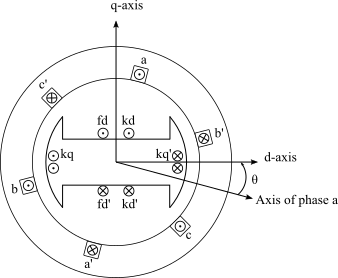
\includegraphics[scale=1]{img/SynchronousGenerator.png} 
	\caption{Schematic diagram of Synchronous Generator}
	\label{fig:SynGenerator}
\end{figure}


We can derive the equations of the synchronous machine similarly to the equations of the magnetic circuit.

The flux linkage for stator phase windings a, b and c are given by
\begin{equation} \label{eq:FluxStator}
	\begin{bmatrix}
		\lambda_a \\
		\lambda_b \\
		\lambda_c
	\end{bmatrix}
	=
	\begin{bmatrix}
		l_{aa} & l_{ab} & l_{ca} & l_{akq1} & l_{akq2} & l_{afd} & l_{akd} \\  
		l_{ab} & l_{bb} & l_{bc} & l_{bkq1} & l_{bkq2} & l_{bfd} & l_{bkd} \\  
		l_{ca} & l_{bc} & l_{cc} & l_{ckq1} & l_{ckq2} & l_{cfd} & l_{ckd} \\  
	\end{bmatrix}
	\begin{bmatrix}
		i_a \\
		i_b \\
		i_c \\
		i_{kq1} \\
		i_{kq2} \\
		i_{fd} \\
		i_{kd} \\
	\end{bmatrix}
\end{equation}

where

$l_{aa}$, $l_{bb}$ and $l_{cc}$ are the self-inductances of the stator windings;

$l_{ab}$, $l_{bc}$ and $l_{ca}$ are the mutual inductances between the stator windings;

$l_{akq1}$, $l_{akq2}$, $l_{afd}$ and $l_{akd}$ are the mutual inductances between stator and rotor windings;

$i_a$, $i_b$ and $i_c$ are the instantaneous stator currents in phases a, b and c;

$i_{kq1}$, $i_{kq2}$, $i_{fd}$ and $i_{kd}$ are the field and amortisseur circuit currents.
 
The equations of the stator phase to neutral voltages are

\begin{equation} \label{eq:VotlageStator}
	\begin{bmatrix}
		v_a \\
		v_b \\
		v_c
	\end{bmatrix}
	=
	\frac{d}{dt}
	\begin{bmatrix}
		\lambda_a \\
		\lambda_b \\
		\lambda_c
	\end{bmatrix}
	-R_a
	\begin{bmatrix}
		i_a \\
		i_b \\
		i_c
	\end{bmatrix}
\end{equation}

where $R_a$ is the armature resistance per phase.

It is important to notice that the inductances are time-varying. They vary with the rotor position, due to the variation in the reluctance of the magnetic flux path (non-uniform air gap). 

The permeance of the magnetic flux path $P$ (inverse of the reluctance $\Re$) in function of the rotor position $\alpha$ can be writen as

\begin{equation}
	P = P_0 + P_2 \cos 2 \alpha
\end{equation}

Inductance is directly proportional to permeance and the relative position between the phase a and the rotor is $\theta$. Therefore, we can write the self-inductance $l_{aa}$ as in equation \ref{eq:SelfInductanceA}. Knowing that the windings of phases b and c are identical to phase a and displaced from it by  $120^{\circ}$ and $240^{\circ}$ respectively, we can also determine the self-inductances $l_{bb}$ and $l_{cc}$. A more detailed derivation of the self-inductances is in \cite{kundur1994power}.

\begin{equation} \label{eq:SelfInductanceA}
	l_{aa} = L_{aa0} - L_{aa2} \cos 2 \theta
\end{equation}
\begin{equation} \label{eq:SelfInductanceB}
	l_{bb} = L_{aa0} - L_{aa2} \cos 2 (\theta - \frac{2 \pi}{3})
\end{equation}
\begin{equation} \label{eq:SelfInductanceC}
	l_{cc} = L_{aa0} - L_{aa2} \cos 2 (\theta + \frac{2 \pi}{3})
\end{equation}

The mutual inductance between two stator windings can be deduced evaluating the flux linking one phase due to the current in the other phase. The mutual inductance will also have a second harmonic variation due to the non-uniform air gap.

\begin{equation} \label{eq:MutualInductanceAB}
	l_{ab} = -L_{ab0} - L_{aa2} \cos 2(\theta + \frac{\pi}{3})
\end{equation}
\begin{equation} \label{eq:MutualInductanceBC}
	l_{bc} = -L_{ab0} - L_{aa2} \cos 2(\theta + \pi)
\end{equation}
\begin{equation} \label{eq:MutualInductanceCA}
	l_{ca} = - L_{ab0} - L_{aa2} \cos 2(\theta + \frac{\pi}{3})
\end{equation}

The rotor circuits see a constant reluctance. The variation in time for the mutual inductances between rotor and stator are due to their relative position. The inductance is maximum when stator and rotor are lined up and zero when they are displaced by $90^{\circ}$.

\begin{equation}
	l_{akq1} = L_{akq1} \cos \theta
\end{equation}
\begin{equation}
	l_{akq2} = L_{akq2} \cos \theta
\end{equation}
\begin{equation}
	l_{afd} = L_{afd} \sin \theta
\end{equation}
\begin{equation}
	l_{akd} = L_{akd} \sin \theta
\end{equation}

Similarly, the mutual inductances between phase b and rotor windings and phase c and rotor windings are defined as

\begin{equation}
	l_{bkq1} = L_{akq1} \cos (\theta - \dfrac{2 \pi}{3})
\end{equation}
\begin{equation}
	l_{bkq2} = L_{akq2} \cos (\theta - \dfrac{2 \pi}{3})
\end{equation}
\begin{equation}
	l_{bfd} = L_{afd} \sin (\theta - \dfrac{2 \pi}{3})
\end{equation}
\begin{equation}
	l_{bkd} = L_{akd} \sin (\theta - \dfrac{2 \pi}{3})
\end{equation}

\begin{equation}
	l_{ckq1} = L_{akq1} \cos (\theta + \dfrac{2 \pi}{3})
\end{equation}
\begin{equation}
	l_{ckq2} = L_{akq2} \cos (\theta + \dfrac{2 \pi}{3})
\end{equation}
\begin{equation}
	l_{cfd} = L_{afd} \sin (\theta + \dfrac{2 \pi}{3})
\end{equation}
\begin{equation}
	l_{ckd} = L_{akd} \sin (\theta + \dfrac{2 \pi}{3})
\end{equation}

The self-inductances of the rotor circuit and the mutual inductance between rotor windings do not vary with the rotor position, since the rotos circuits see constant reluctance. Therefore, the flux linkage for the rotor windings are given by

\begin{equation} \label{eq:FluxRotor}
	\begin{bmatrix}
		\lambda_{kq1} \\
		\lambda_{kq2} \\
		\lambda_{fd} \\
		\lambda_{kd} \\
	\end{bmatrix}
	=
	\begin{bmatrix}
		l_{akq1} & l_{bkq1} & l_{ckq1} & L_{kq1} & L_{kq1kq2} & 0 & 0 \\  
		l_{akq2} & l_{bkq2} & l_{ckq2} & L_{kq1kq2} & L_{kq2} & 0 & 0 \\ 
		l_{afd} & l_{bfd} & l_{cfd} & 0 & 0 & L_{fd} & L_{fdkd} \\
		l_{akd} & l_{bkd} & l_{ckd} & 0 & 0 & L_{fdkd} & L_{kd} \\  
	\end{bmatrix}
	\begin{bmatrix}
		i_a \\
		i_b \\
		i_c \\
		i_{kq1} \\
		i_{kq2} \\
		i_{fd} \\
		i_{kd}
	\end{bmatrix}
\end{equation}

The rotor voltage equations are

\begin{equation} \label{eq:VotlageRotor}
	\begin{bmatrix}
		v_{kq1} \\
		v_{kq2} \\
		v_{fd} \\
		v_{kd}
	\end{bmatrix}
	=
	\frac{d}{dt}
	\begin{bmatrix}
		\lambda_{kq1} \\
		\lambda_{kq2} \\
		\lambda_{fd} \\
		\lambda_{kd}
	\end{bmatrix}
	+
	\begin{bmatrix}
		R_{kq1} & 0 & 0 & 0 \\
		0 & R_{kq2} & 0 & 0 \\
		0 & 0 & R_{fd} & 0 \\
		0 & 0 & 0 & R_{kd}
	\end{bmatrix}
	\begin{bmatrix}
		i_{kq1} \\
		i_{kq2} \\
		i_{fd} \\
		i_{kd}
	\end{bmatrix}
\end{equation}

Replacing the inductances values in equations \ref{eq:FluxStator} and \ref{eq:FluxRotor}, we can write the flux equation as in equation \ref{eq:FluxRotorStator}. The flux equation together with the voltage equations \ref{eq:VotlageStator} and \ref{eq:VotlageRotor} completely describe the electrical performance of a synchronous machine.

\begin{equation} \label{eq:FluxRotorStator}
	\begin{bmatrix}
		\boldsymbol{\lambda}_{abcs} \\
		\boldsymbol{\lambda}_{dqr}
	\end{bmatrix}
	=
	\begin{bmatrix}
		\mathbf{L}_s & \mathbf{L}_{rs} \\
		\mathbf{L}_{rs}^{T} & \mathbf{L}_r
	\end{bmatrix}
	\begin{bmatrix}
		\mathbf{i}_{abcs} \\
		\mathbf{i}_{dqr}
	\end{bmatrix}
\end{equation}

Where

\begin{equation}
	\mathbf{L}_s
	=
	\begin{bmatrix}
		L_{aa0} - L_{aa2} \cos 2 \theta &
		-L_{ab0} - L_{aa2} \cos 2(\theta - \dfrac{\pi}{3}) &
		-L_{ab0} - L_{aa2}\cos 2(\theta + \dfrac{\pi}{3}) &\\[6pt]
		-L_{ab0} - L_{aa2} \cos 2(\theta - \dfrac{\pi}{3}) &
		L_{aa0} - L_{aa2} \cos 2(\theta - \dfrac{2 \pi}{3})&
		-L_{ab0} - L_{aa2}\cos 2(\theta + \pi) \\[6pt]
		-L_{ab0} - L_{aa2} \cos 2(\theta + \dfrac{\pi}{3}) &
		-L_{ab0} - L_{aa2} \cos 2(\theta + \pi)&
		L_{aa0} - L_{aa2}\cos 2(\theta + \dfrac{2 \pi}{3}) \\[6pt]
	\end{bmatrix}
\end{equation}

\begin{equation}
	\mathbf{L}_{rs}
	=
	\begin{bmatrix}
		L_{akq1} \cos \theta &
		L_{akq2} \cos \theta &
		L_{afd} \sin \theta &
		L_{akd} \sin \theta \\[6pt]
		L_{akq1} \cos (\theta - \dfrac{2 \pi}{3}) &
		L_{akq2} \cos (\theta - \dfrac{2 \pi}{3}) &
		L_{afd} \sin (\theta - \dfrac{2 \pi}{3}) &
		L_{akd} \sin (\theta - \dfrac{2 \pi}{3}) \\[6pt]
		L_{akq1} \cos (\theta + \dfrac{2 \pi}{3}) &
		L_{akq2} \cos (\theta + \dfrac{2 \pi}{3}) &
		L_{afd} \sin (\theta + \dfrac{2 \pi}{3}) &
		L_{akd} \sin (\theta + \dfrac{2 \pi}{3}) \\[6pt]
	\end{bmatrix}
\end{equation}

\begin{equation}
	\mathbf{L}_r
	=
	\begin{bmatrix}
		L_{kq1} & L_{kq1kq2} & 0 & 0 \\  
		L_{kq1kq2} & L_{kq2} & 0 & 0 \\ 
		0 & 0 & L_{fd} & L_{fdkd} \\
		0 & 0 & L_{fdkd} & L_{kd} \\  
	\end{bmatrix}
\end{equation}

\begin{align}
   \mathbf{i}_{abcs} &= 
  \begin{bmatrix}
    i_{a} & i_{b} & i_{c}
  \end{bmatrix}^T \\
  %  
  \mathbf{i}_{qdr} &= 
  \begin{bmatrix}
    i_{kq1} & i_{kq2} & i_{fd} & i_{kd}
  \end{bmatrix}^T \\
  %
  \boldsymbol{\lambda}_{abcs} &= 
  \begin{bmatrix}
    \lambda_{a} & \lambda_{b} & \lambda_{c}
  \end{bmatrix}^T \\
  %  
  \boldsymbol{\lambda}_{dqr} &= 
  \begin{bmatrix}
     \lambda_{kq1} & \lambda_{kq2} & \lambda_{fd} & \lambda_{kd} 
  \end{bmatrix}^T \\
 \end{align}


The mechanical equations are:
%
\begin{align}
\frac{d\theta_r}{dt} &= \omega_r \label{eq:d_theta} \\
\frac{d\omega_r}{dt} &= \frac{P}{2J} (T_e-T_m) \label{eq:d_omega}
\end{align}
%
where $\theta_r$ is the rotor position, $\omega_r$ is the angular electrical speed, $P$ is the number of poles, $J$ is the moment of inertia, $T_m$ and $T_e$ are the mechanical and electrical torque, respectively. Motor convention is used for all models. 

\iffalse
\subsection{Model}
The electrical model in the phase domain is described by the following equations:
%
\begin{align}
  \mathbf{v}_{abcs} &= \mathbf{R}_s \mathbf{i}_{abcs} + \frac{d}{dt} \boldsymbol{\lambda}_{abcs} \\
  \mathbf{v}_{qdr} &= \mathbf{R}_r \mathbf{i}_{qdr} + \frac{d}{dt}  \boldsymbol{\lambda}_{qdr}
\end{align}
%
where
%
\begin{align}
  \mathbf{v}_{abcs} &= 
  \begin{pmatrix}
    v_{as} & v_{bs} & v_{cs}
  \end{pmatrix}^T \\
  %  
  \mathbf{v}_{qdr} &= 
  \begin{pmatrix}
    v_{kq1} & v_{kq2} & v_{fd} & v_{kd} 
  \end{pmatrix}^T \\
  %
  \mathbf{i}_{abcs} &= 
  \begin{pmatrix}
    i_{as} & i_{bs} & i_{cs}
  \end{pmatrix}^T \\
  %  
  \mathbf{i}_{qdr} &= 
  \begin{pmatrix}
    i_{kq1} & i_{kq2} & i_{fd} & i_{kd} 
  \end{pmatrix}^T \\
  %
  \boldsymbol{\lambda}_{abcs} &= 
  \begin{pmatrix}
    \lambda_{as} & \lambda_{bs} & \lambda_{cs}
  \end{pmatrix}^T \\
  %  
  \boldsymbol{\lambda}_{qdr} &= 
  \begin{pmatrix}
    \lambda_{kq1} & \lambda_{kq2} & \lambda_{fd} & \lambda_{kd} 
  \end{pmatrix}^T \\
  %
  \mathbf{R}_s &= diag
  \begin{bmatrix}
    r_s & r_s & r_s 
  \end{bmatrix} \\
  %
  \mathbf{R}_r &= diag
  \begin{bmatrix}
    r_{kq1} & r_{kq2} & r_{fd} & r_{kd}
  \end{bmatrix}
\end{align}
%
The flux linkages are:
%
\begin{align}
  \boldsymbol{\lambda}_{abcs} &= \mathbf{L}_{ss} \mathbf{i}_{abcs} + \mathbf{L}_{sr} \mathbf{i}_{qdr}  \\
  \boldsymbol{\lambda}_{qdr} &= \mathbf{L}_{rs} \mathbf{i}_{abcs} + \mathbf{L}_{rr} \mathbf{i}_{qdr}
\end{align}
%
where the inductances are time variant variables as defined in \cite{krause2002sudhoff}.
TODO: electromagnetic torque
\fi

\subsubsection{Equations in Rotor Reference Frame}

This section depicts the synchronous generator equations in terms of machine variables referred to the stator windings which is indicated by the prime symbol. Due to the transform of the stator variables to the rotor reference frame, the stator equations change, whereas the rotor equations remain the same.
%
\begin{equation}
  \begin{pmatrix}
    \mathbf{v}_{qd0s} \\
    \mathbf{v}_{qdr}
  \end{pmatrix}
  =  
  \mathbf{R}'
  \begin{pmatrix}
    \mathbf{i}_{qd0s} \\
    \mathbf{i}_{qdr}'
  \end{pmatrix}
  +
  \frac{d}{dt}
  \begin{pmatrix}
    \boldsymbol{\lambda}_{qd0s} \\
    \boldsymbol{\lambda}_{qdr}'
  \end{pmatrix}
  + \omega_r
  \begin{pmatrix}
    \boldsymbol{\lambda}_{dqs} \\
    0
  \end{pmatrix}
\end{equation}
%
where
%
\begin{align}
  \mathbf{R}' &= diag
  \begin{bmatrix}
    r_s & r_s & r_s & r_{kq1}' & r_{kq2}' & r_{fd}' & r_{kd}' 
  \end{bmatrix} \\
  \boldsymbol{\lambda}_{dqs} &= 
  \begin{pmatrix}
    \lambda_{ds} & -\lambda_{qs} & 0
  \end{pmatrix}^T
\end{align}
%
The flux linkages are:
%
\begin{equation}
  \begin{pmatrix}
    \boldsymbol{\lambda}_{qd0s} \\
    \boldsymbol{\lambda}_{qdr}'
  \end{pmatrix}
  =
  \begin{bmatrix}
    \mathbf{L}_{qdss} & \mathbf{L}_{qdsr}' \\
    \mathbf{L}_{qdrs}' & \mathbf{L}_{rr}'    
  \end{bmatrix}
  \begin{pmatrix}
    \mathbf{i}_{qd0s} \\
    \mathbf{i}_{qdr}'
  \end{pmatrix}
  \label{eq:flux}
\end{equation}
%
where
%
\begin{align}
  \mathbf{L}_{qdss} &= 
  \begin{bmatrix}
    L_{q} & 0 & 0 \\
    0 & L_{d} & 0 \\
    0 & 0 & L_{ls}
  \end{bmatrix} \\
  %  
  \mathbf{L}_{qdsr}' &= 
  \begin{bmatrix}
    L_{mq} & L_{mq} & 0 & 0 \\
    0 & 0 & L_{md} & L_{md} \\
    0 & 0 & 0 & 0
  \end{bmatrix} \\
  %
  \mathbf{L}_{qdrs}' &=
  \begin{bmatrix}
    L_{mq} & 0 & 0 \\
    L_{mq} & 0 & 0 \\
    0 & L_{md} & 0 \\
    0 & L_{md} & 0
  \end{bmatrix} \\
  %
  \mathbf{L}_{rr}' &=
  \begin{bmatrix}
    L_{kq1}' & L_{mq} & 0 & 0 \\
    L_{mq} & L_{kq2}' & 0 & 0 \\
    0 & 0 & L_{fd}' & L_{md} \\
    0 & 0 & L_{md} & L_{kd}'
  \end{bmatrix} \\
  %
\end{align}
%
with 
%
\begin{align}
  L_{q} &= L_{ls} + L_{mq} \\
  L_{d} &= L_{ls} + L_{md} \\
  L_{kq1'} &= L_{lkq1'} + L_{mq} \\
  L_{kq2'} &= L_{lkq2'} + L_{mq} \\
  L_{fd'} &= L_{lfd'} + L_{md} \\
  L_{kd'} &= L_{lkd'} + L_{md}
\end{align}

\subsubsection{State Space Model}
The flux linkage variables are chosen as electrical states of the state-space representation. Then, the currents can be calculated from equation \ref{eq:flux}.
%
\begin{equation}
  \frac{d}{dt}
  \begin{pmatrix}
    \boldsymbol{\lambda}_{qd0s} \\
    \boldsymbol{\lambda}_{qdr}'
  \end{pmatrix}
  =
  \begin{pmatrix}
    \mathbf{v}_{qd0s} \\
    \mathbf{v}_{qdr}'
  \end{pmatrix}
  - \mathbf{R}'
  \begin{pmatrix}
    \mathbf{i}_{qd0s} \\
    \mathbf{i}_{qdr}'
  \end{pmatrix}
  - \omega_r
  \begin{pmatrix}
    \boldsymbol{\lambda}_{dqs} \\
    0
  \end{pmatrix}
\end{equation}
%
or
%
\begin{equation}
  \frac{d}{dt}
  \begin{pmatrix}
    \boldsymbol{\lambda}_{qd0s} \\
    \boldsymbol{\lambda}_{qdr}'
  \end{pmatrix}
  =
  \begin{pmatrix}
    \mathbf{v}_{qd0s} \\
    \mathbf{v}_{qdr}'
  \end{pmatrix}
  - \mathbf{R}'
  \begin{bmatrix}
    \mathbf{L}_{qdss} & \mathbf{L}_{qdsr}' \\
    \mathbf{L}_{qdrs}' & \mathbf{L}_{rr}'    
  \end{bmatrix}^{-1}
  \begin{pmatrix}
    \boldsymbol{\lambda}_{qd0s} \\
    \boldsymbol{\lambda}_{qdr}
  \end{pmatrix}  
    - \omega_r
  \begin{pmatrix}
    \boldsymbol{\lambda}_{dqs} \\
    0
  \end{pmatrix}
\end{equation}
%
since the currents are 
%
\begin{align} 
   \begin{pmatrix}
    \mathbf{i}_{qd0s} \\
    \mathbf{i}_{qdr}'
  \end{pmatrix}
  = 
  \begin{bmatrix}
    \mathbf{L}_{qdss} & \mathbf{L}_{qdsr}' \\
    \mathbf{L}_{qdrs}' & \mathbf{L}_{rr}'    
  \end{bmatrix}^{-1}
  \begin{pmatrix}
    \boldsymbol{\lambda}_{qd0s} \\
    \boldsymbol{\lambda}_{qdr}
  \end{pmatrix}
\end{align}
%
The voltages of the damper windings are always zero since they are short-circuited. The state-space representation of the mechanical part is
%
\begin{align}
 \frac{d}{dt}
  \begin{pmatrix}
    \theta_r \\
    \omega_r
  \end{pmatrix}
  =
  \begin{bmatrix}
    0 & 1 \\
    0 & 0 \\
  \end{bmatrix}
  \begin{pmatrix}
    \theta_r \\
    \omega_r
  \end{pmatrix}
  + 
  \begin{pmatrix}
    0 \\
    \frac{P}{2J} \left( T_e - T_m \right)
  \end{pmatrix} 
\end{align}
%
where the electric torque is
%
\begin{equation}
  T_e = \frac{3P}{4} \left( \boldsymbol{\lambda}_{ds} \mathbf{i}_{qs} - \boldsymbol{\lambda}_{qs} \mathbf{i}_{ds} \right)
\end{equation}
%

\subsubsection{Alternative State Space Representation}
Defining q- and d-axis flux linkages 
%
\begin{align}
  \lambda_{mq} &= L_{mq} \left( i_{qs} + i_{kq1}' + i_{kq2}' \right) \\
  \lambda_{md} &= L_{md} \left( i_{ds} + i_{fd}' + i_{kd}' \right) \\
\end{align}
%
allows to rewrite the equations